\input header 
\begin{document}
\centerline{\textbf{\Large Errors in single layer $|\mathbf{u}^s-\mathbf{u}^s_{ex}|$ -- $O(h^3)$ method}}
\bigskip
%\vskip6.7truecm
\noindent
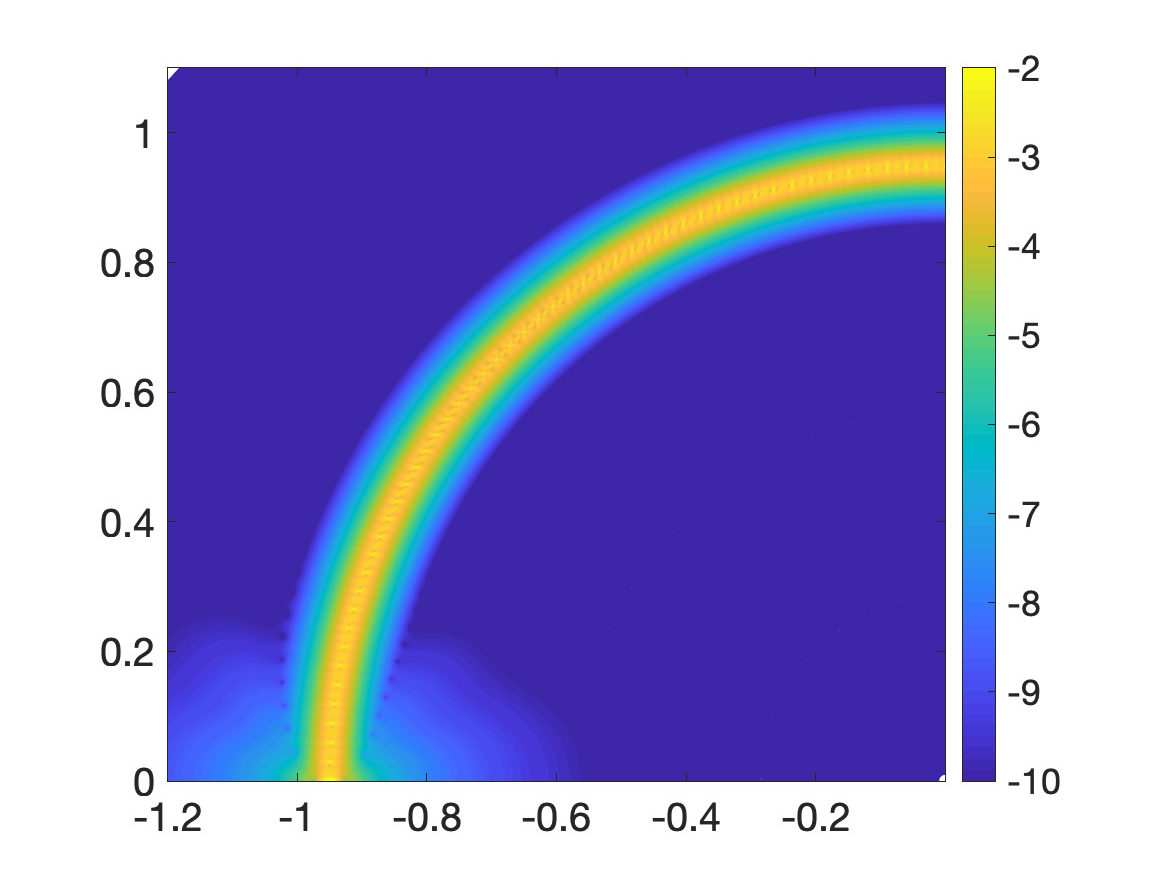
\includegraphics[trim=40 20 40 10, clip, width=2.5truein]{figs/fig100a} 
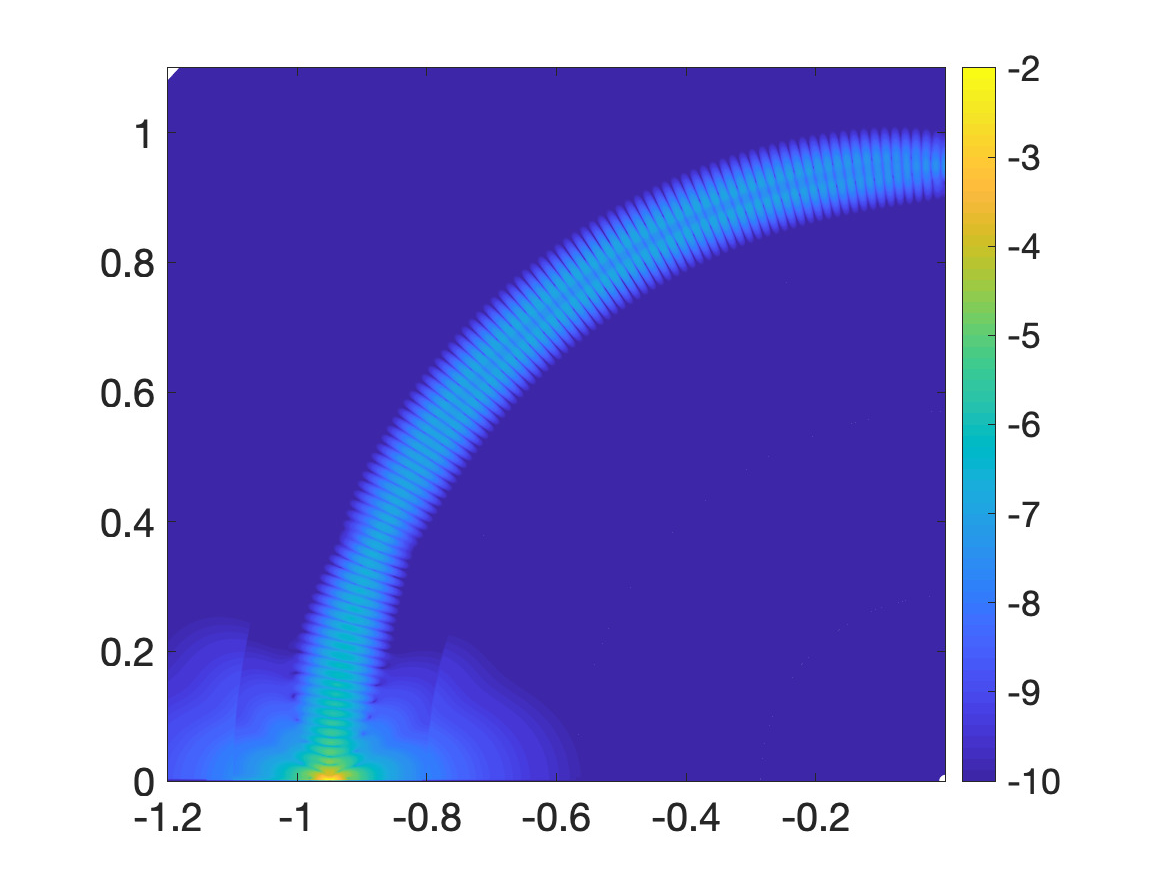
\includegraphics[trim=40 20 40 10, clip, width=2.5truein]{figs/fig100b} 
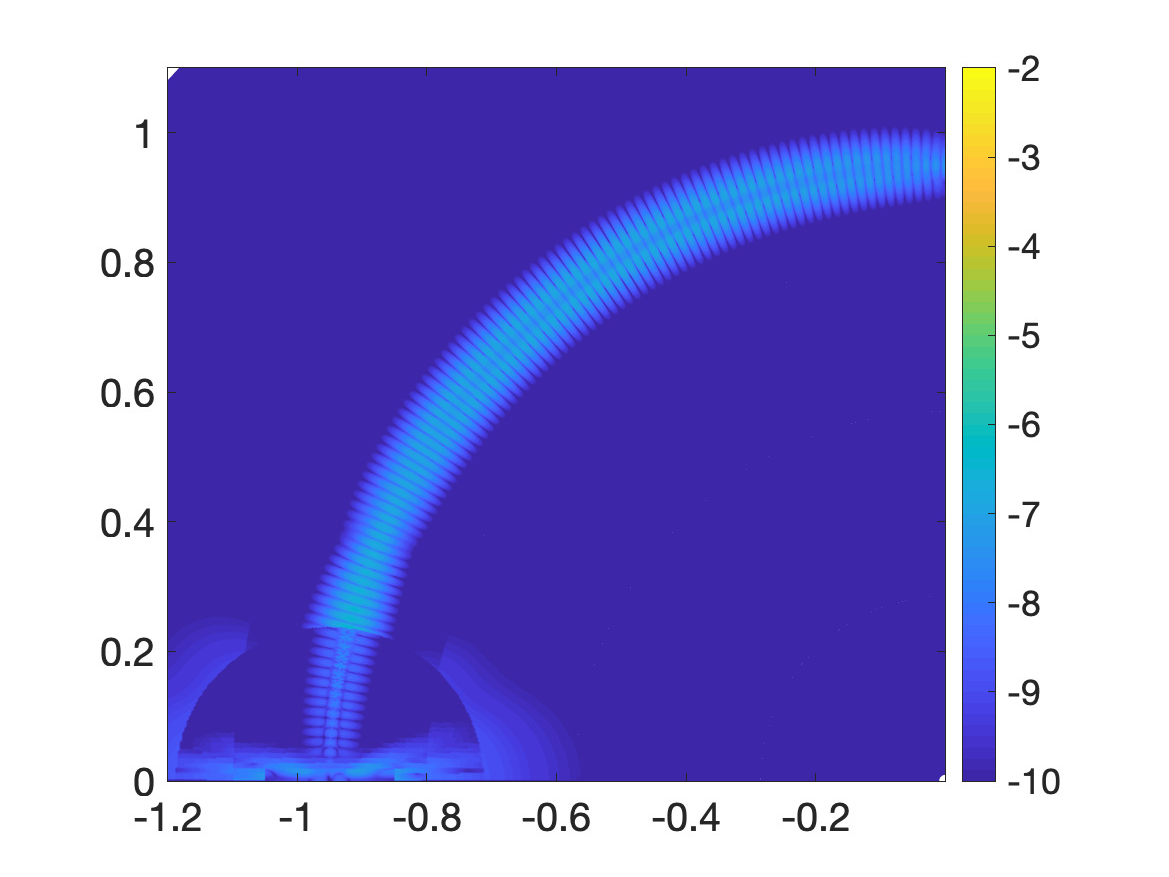
\includegraphics[trim=40 20 40 10, clip, width=2.5truein]{figs/fig100c} \\
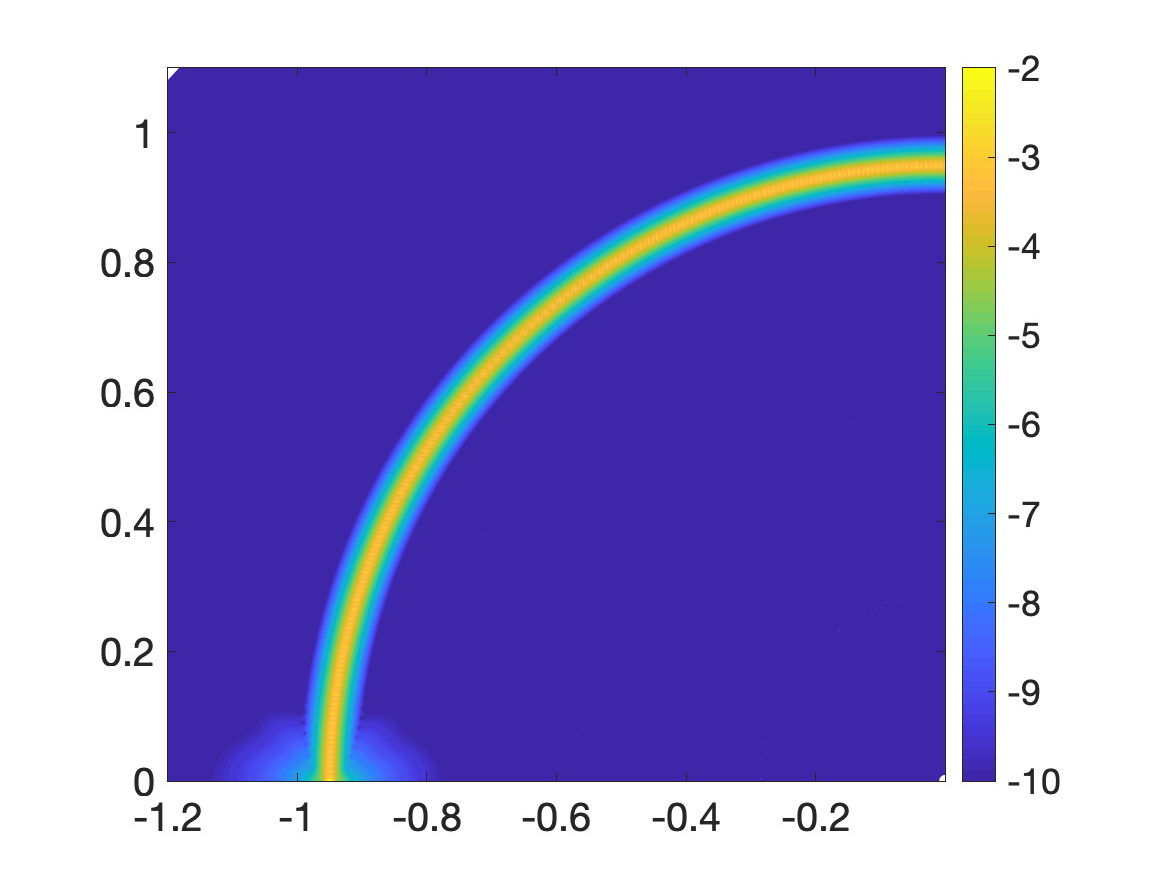
\includegraphics[trim=40 20 40 10, clip, width=2.5truein]{figs/fig200a} 
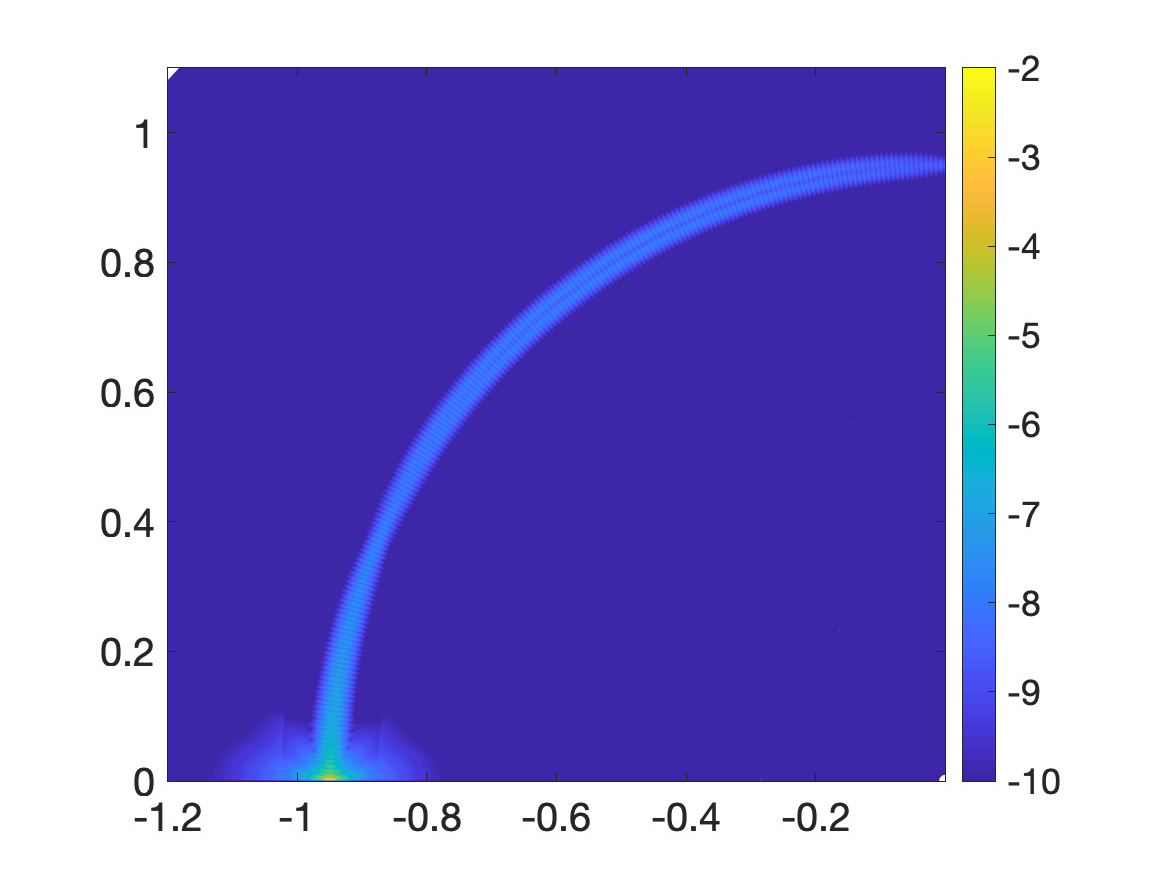
\includegraphics[trim=40 20 40 10, clip, width=2.5truein]{figs/fig200b} 
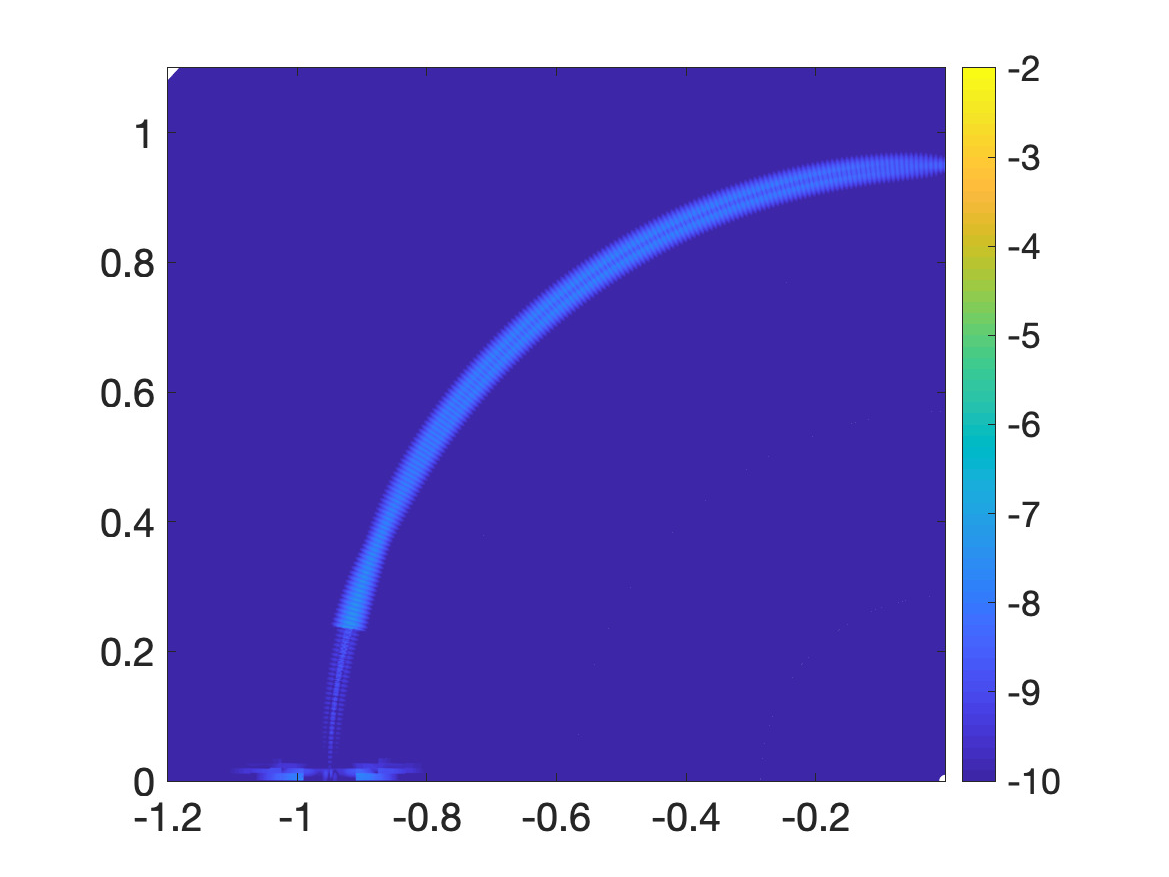
\includegraphics[trim=40 20 40 10, clip, width=2.5truein]{figs/fig200c}\\ 
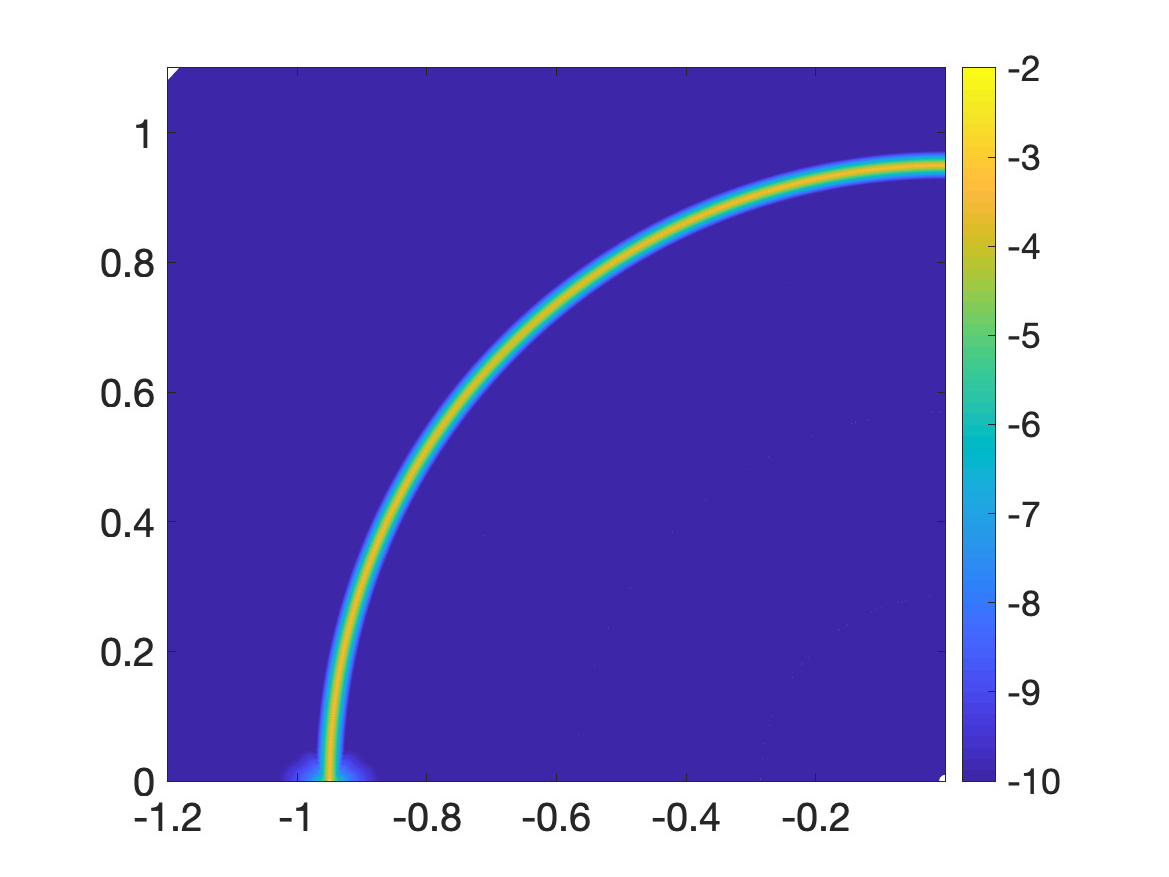
\includegraphics[trim=40 20 40 10, clip, width=2.5truein]{figs/fig400a} 
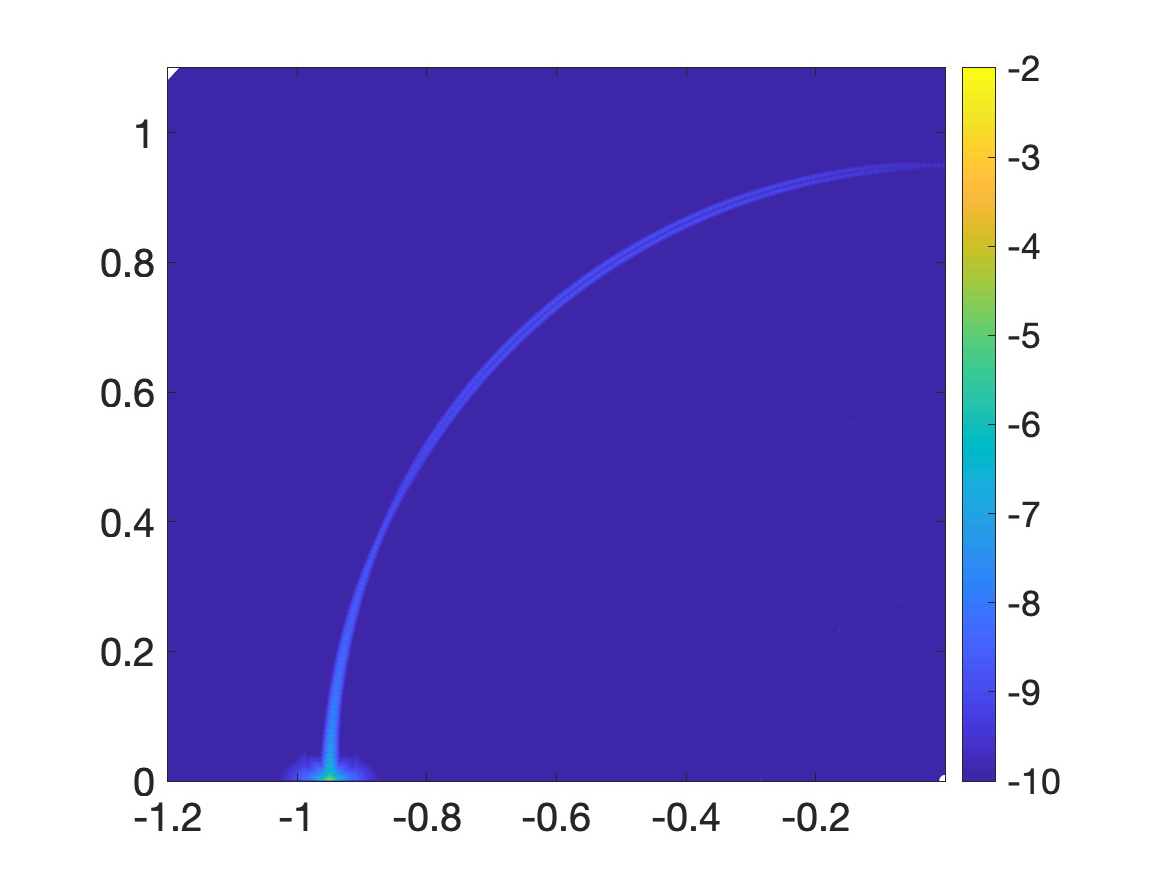
\includegraphics[trim=40 20 40 10, clip, width=2.5truein]{figs/fig400b} 
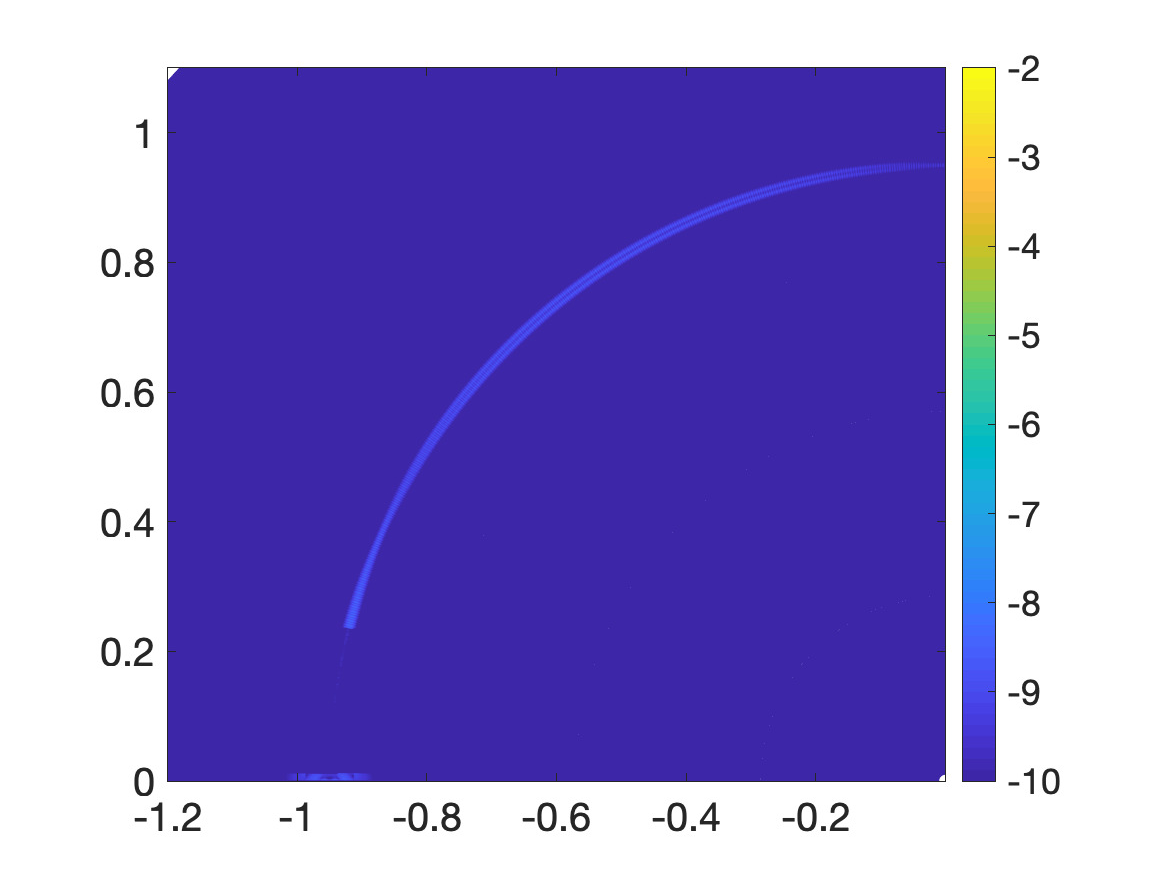
\includegraphics[trim=40 20 40 10, clip, width=2.5truein]{figs/fig400c}\\
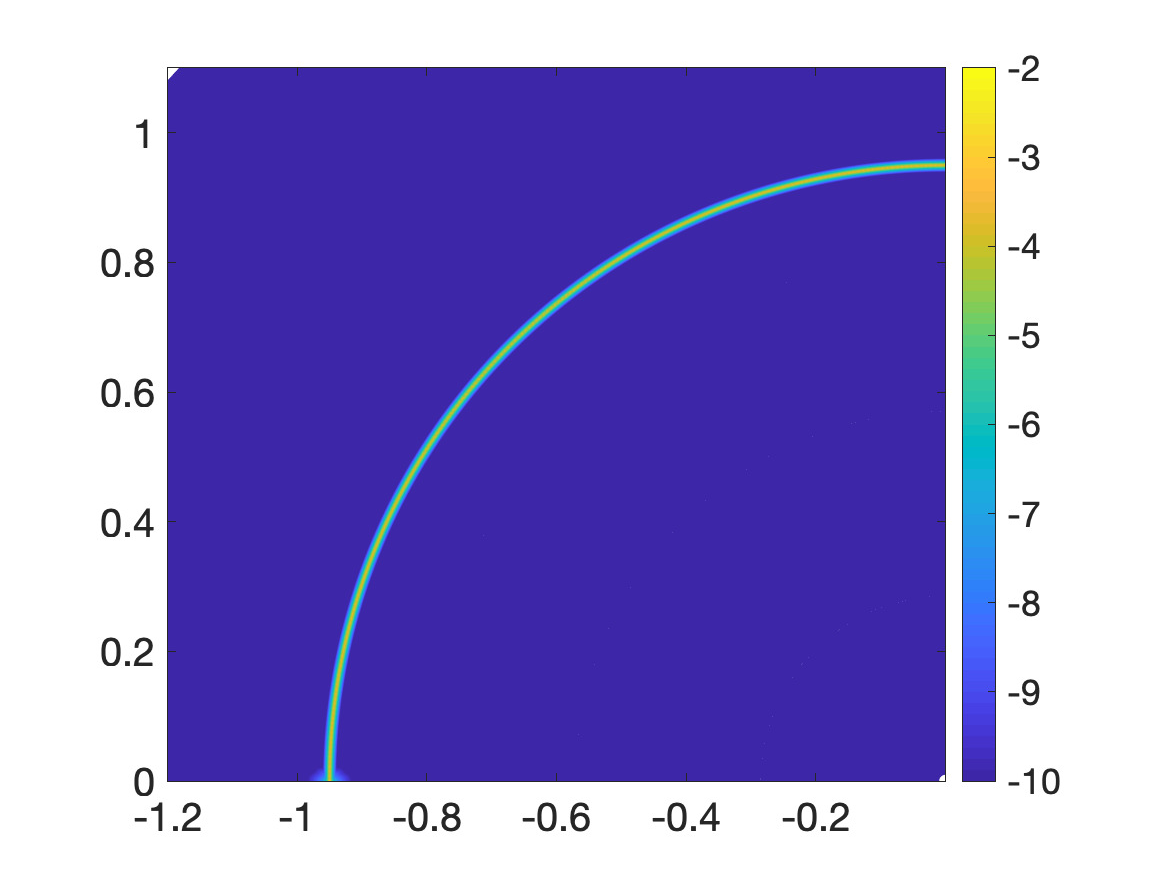
\includegraphics[trim=40 20 40 10, clip, width=2.5truein]{figs/fig800a} 
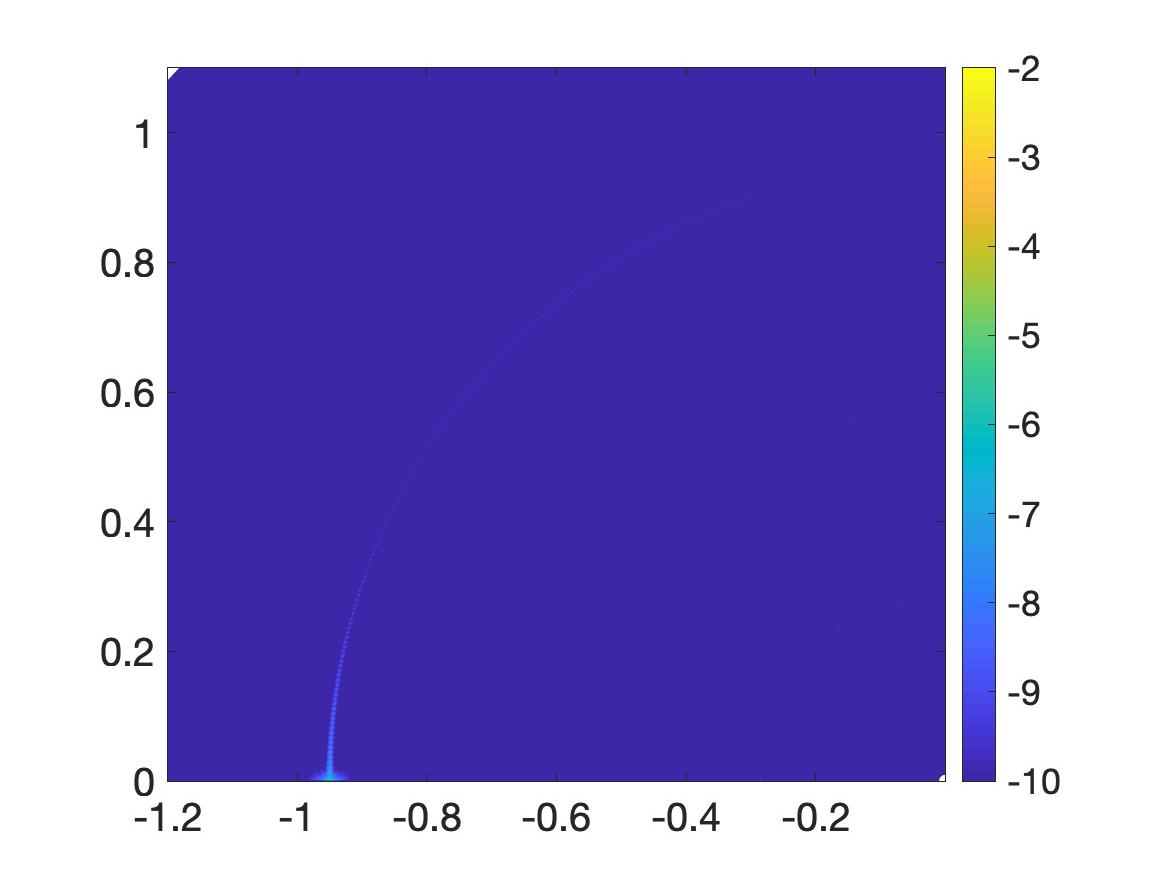
\includegraphics[trim=40 20 40 10, clip, width=2.5truein]{figs/fig800b} 
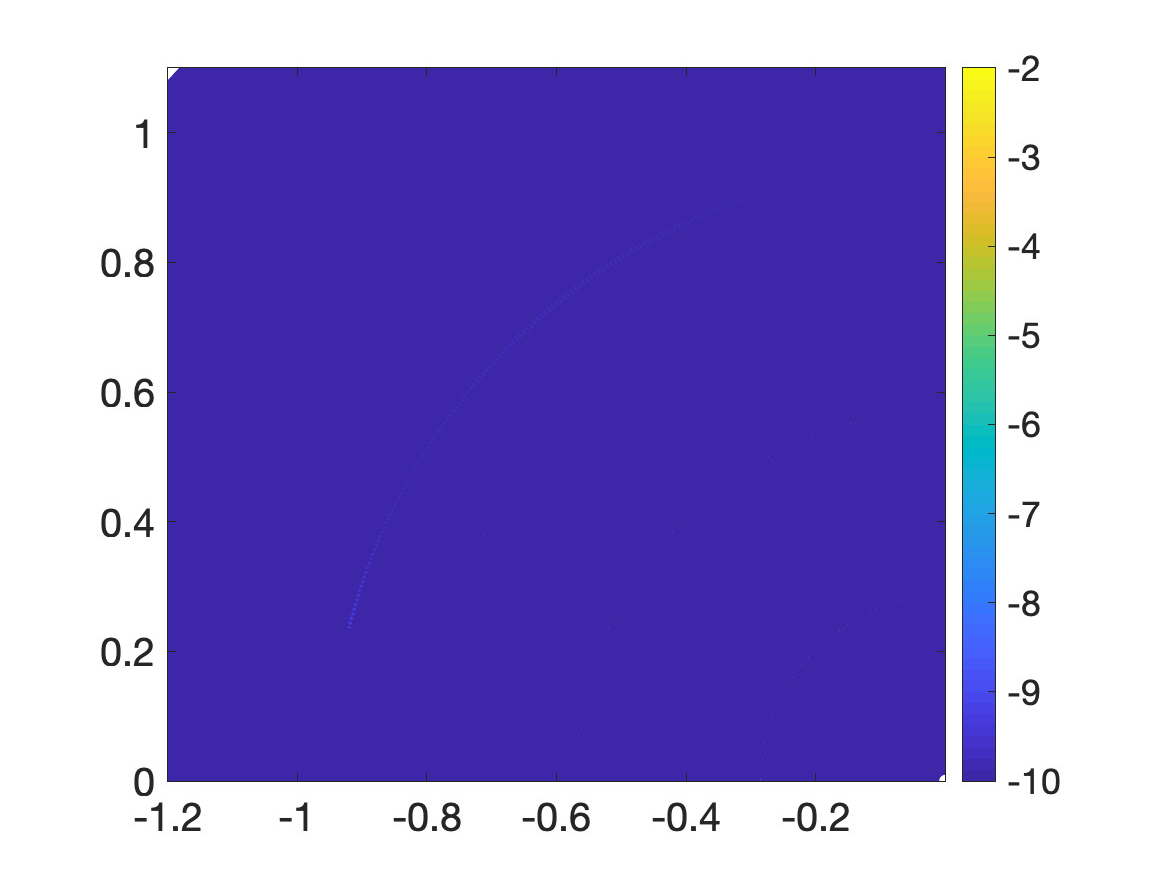
\includegraphics[trim=40 20 40 10, clip, width=2.5truein]{figs/fig800c} 
\vfill
\noindent
The rows, top to bottom, show results using $n=100,200,400,800$.\\
The columns, left to right, show errors obtained with $T[G]$, $T[G]+E[H]$, $T[G]+E[H]+E[B]$.

\newpage
\centerline{\textbf{\Large Errors in single layer $|\mathbf{u}^s-\mathbf{u}^s_{ex}|$ --  $O(h^4)$ method}}
\bigskip
%\vskip6.7truecm
\noindent
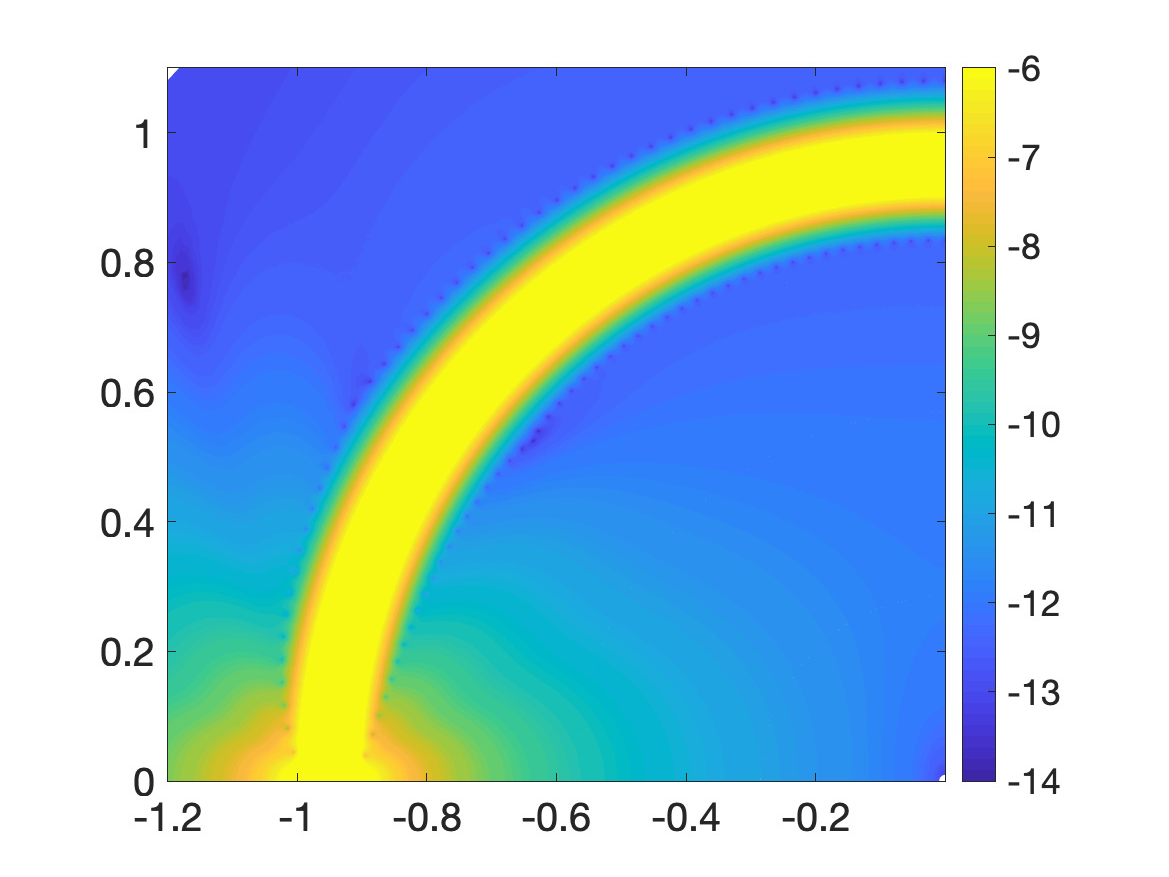
\includegraphics[trim=40 20 40 10, clip, width=2.5truein]{figs/fig100a4} 
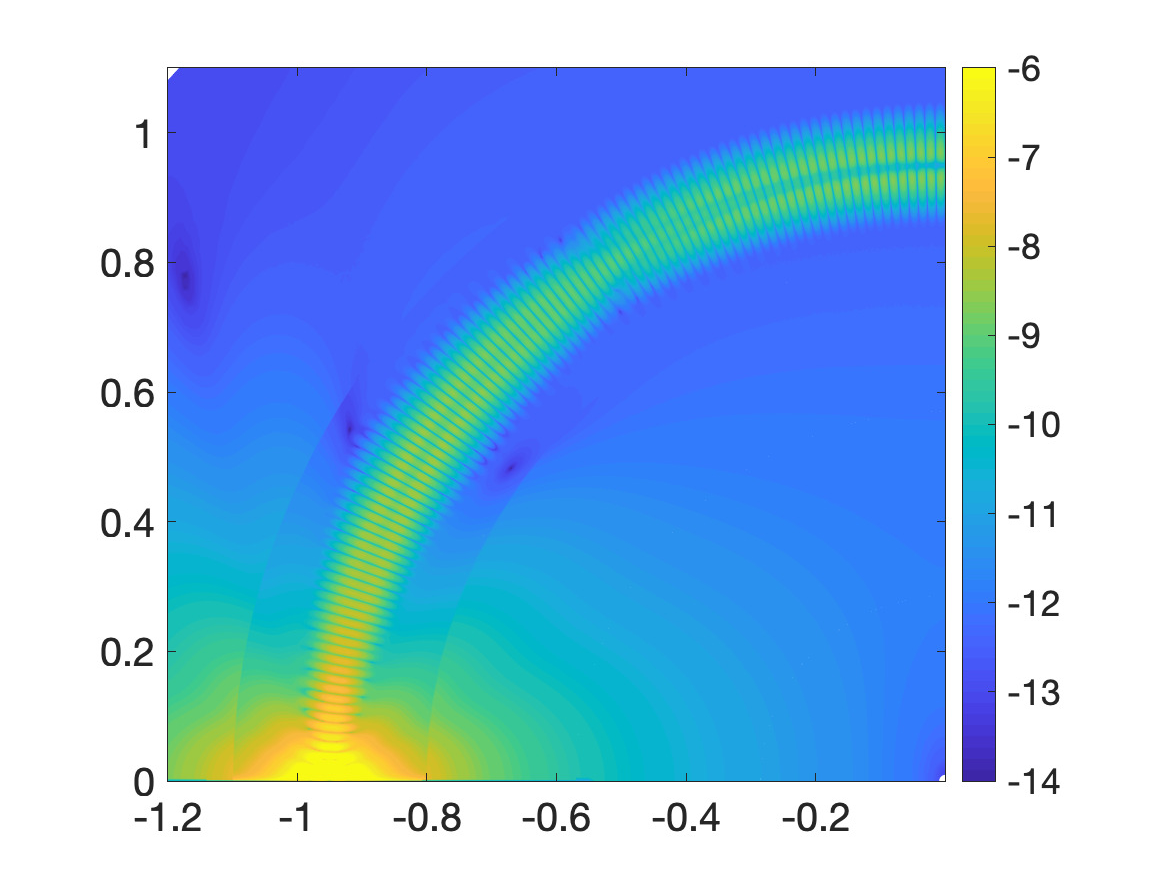
\includegraphics[trim=40 20 40 10, clip, width=2.5truein]{figs/fig100b4} 
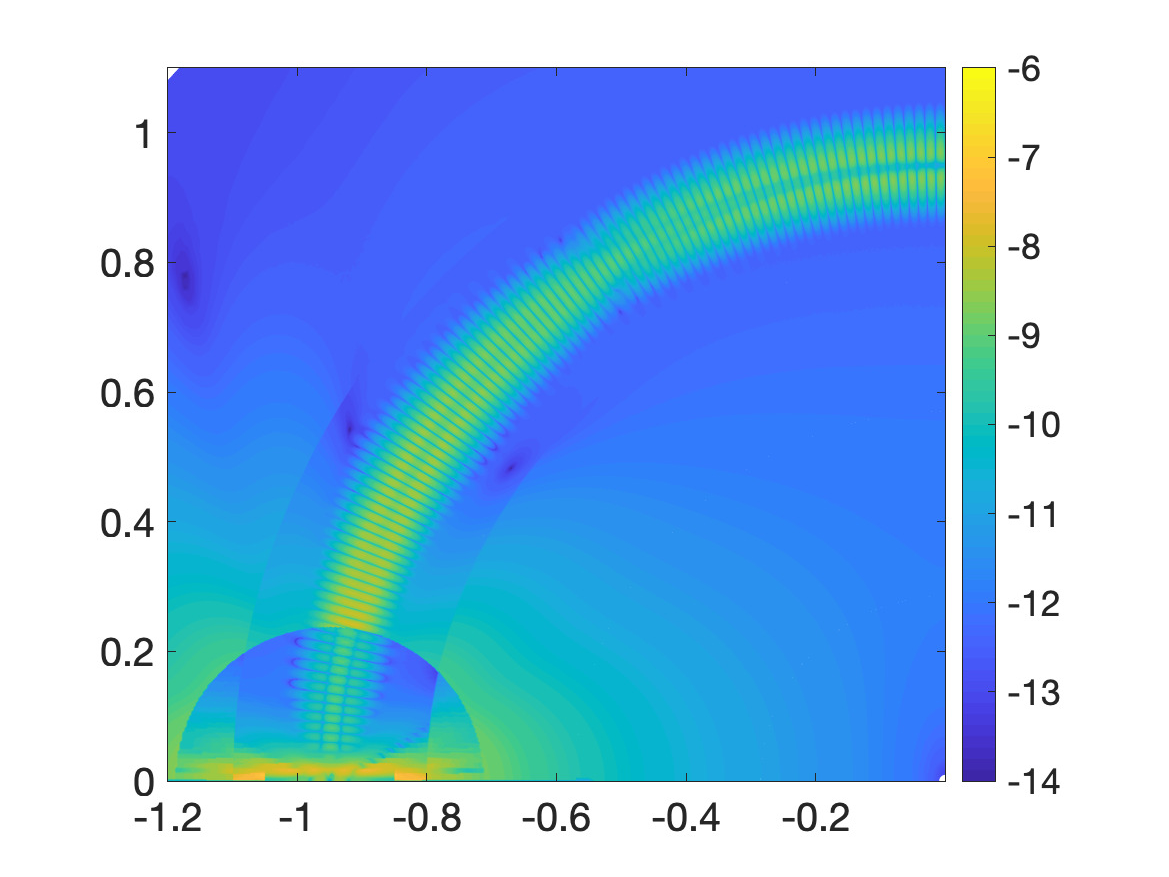
\includegraphics[trim=40 20 40 10, clip, width=2.5truein]{figs/fig100c4} \\
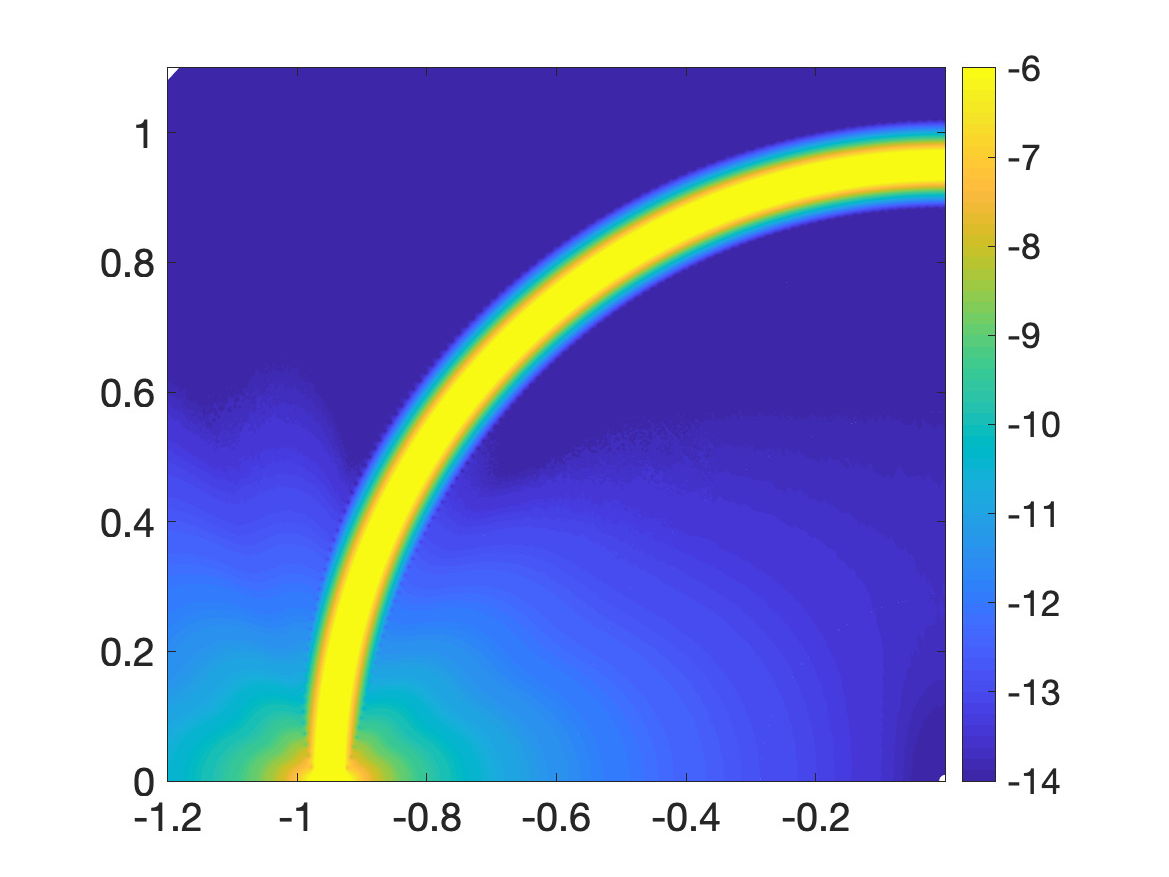
\includegraphics[trim=40 20 40 10, clip, width=2.5truein]{figs/fig200a4} 
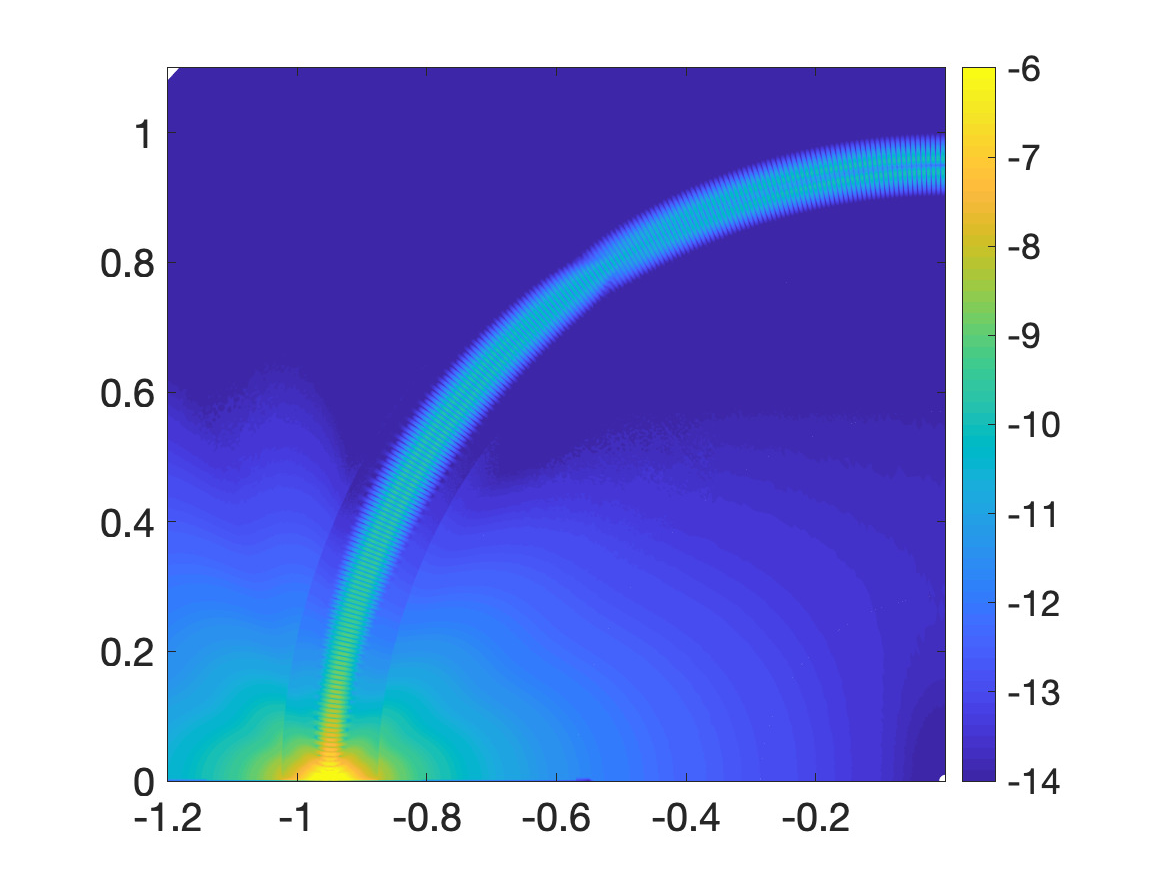
\includegraphics[trim=40 20 40 10, clip, width=2.5truein]{figs/fig200b4} 
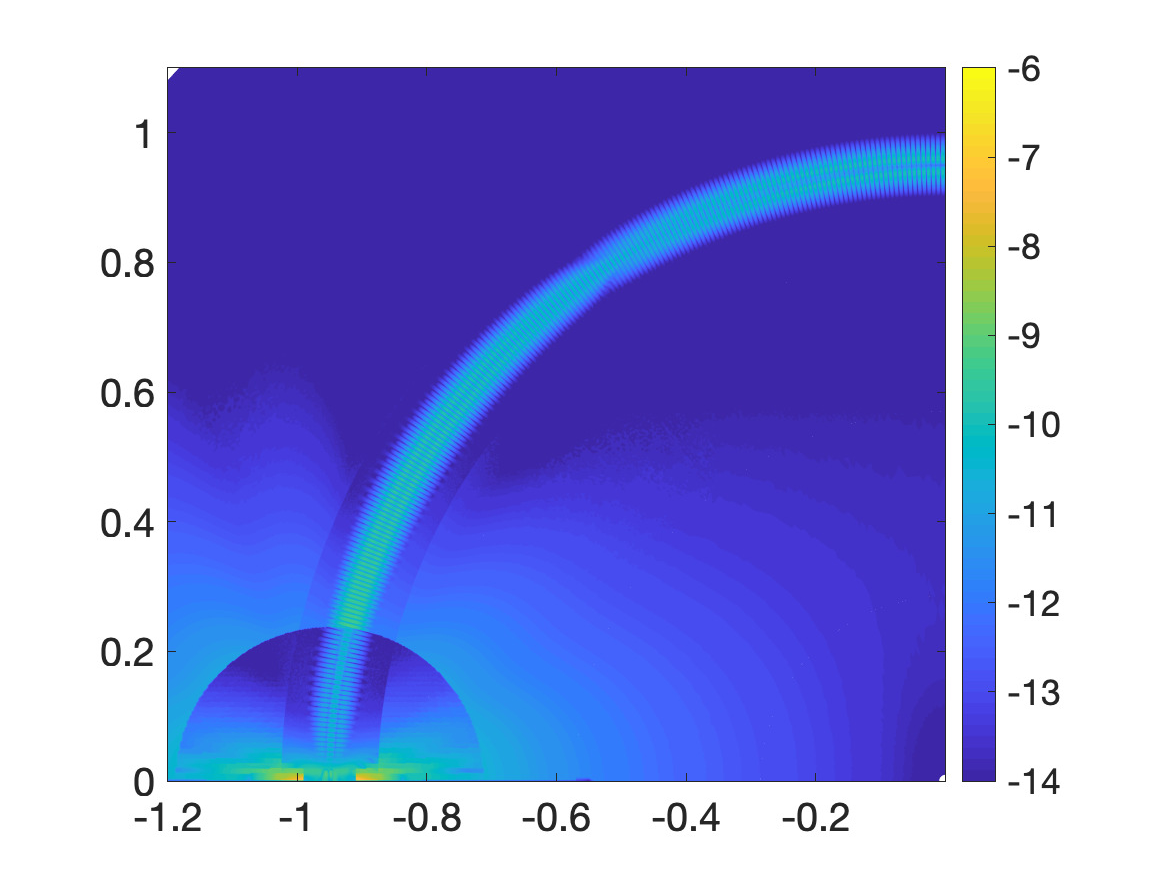
\includegraphics[trim=40 20 40 10, clip, width=2.5truein]{figs/fig200c4}\\ 
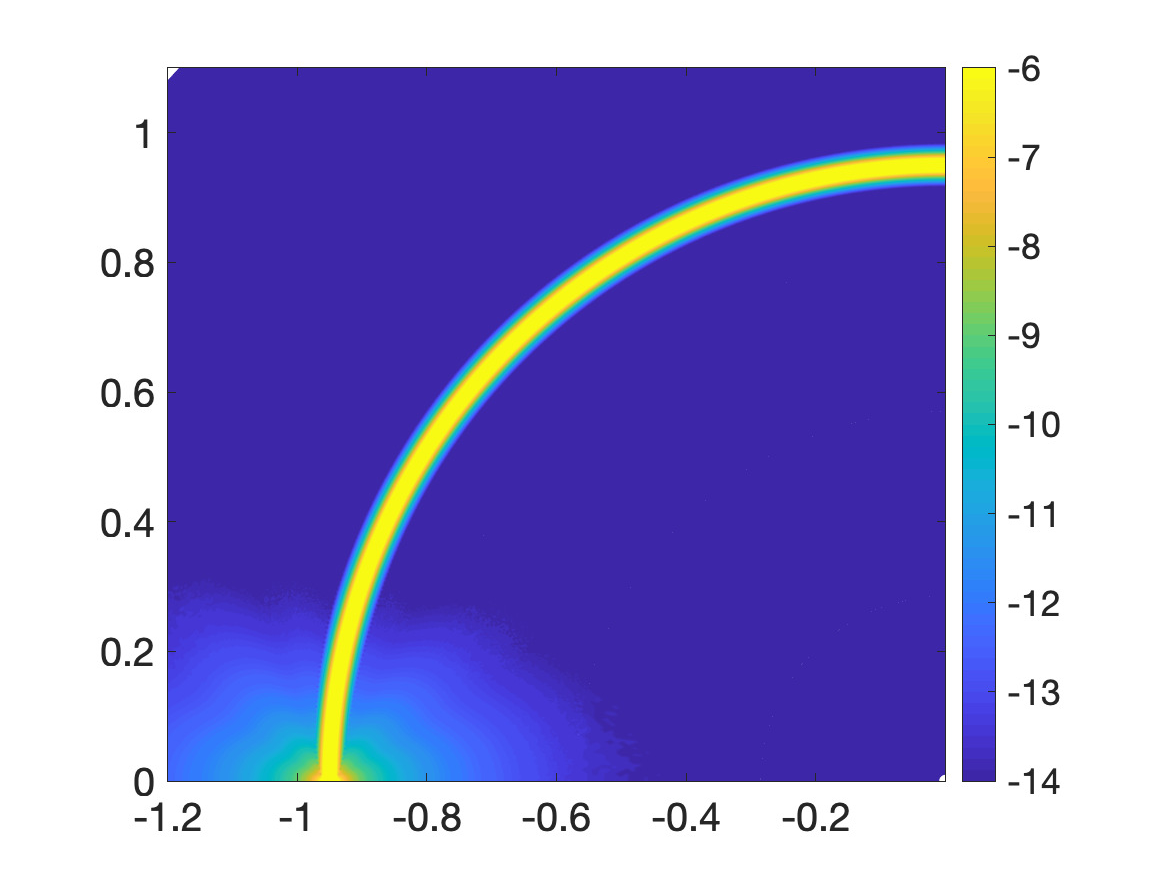
\includegraphics[trim=40 20 40 10, clip, width=2.5truein]{figs/fig400a4} 
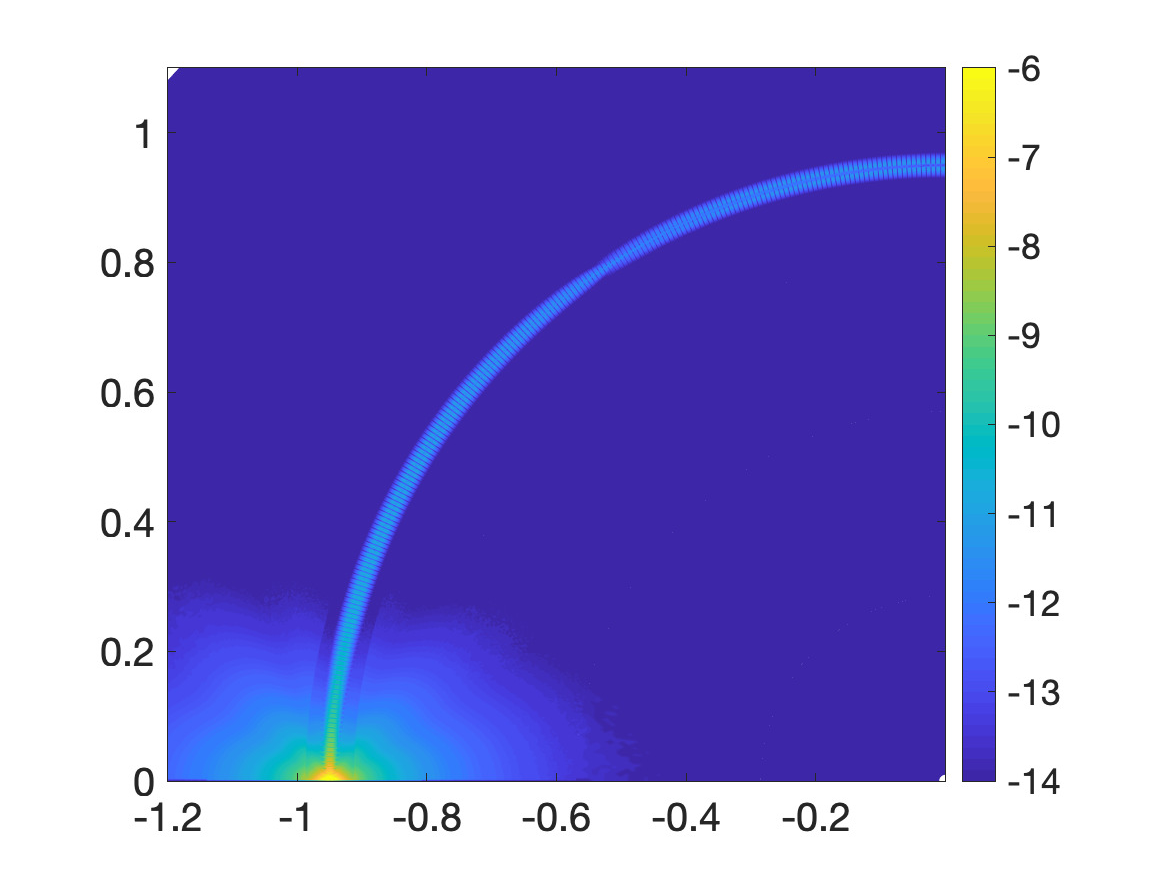
\includegraphics[trim=40 20 40 10, clip, width=2.5truein]{figs/fig400b4} 
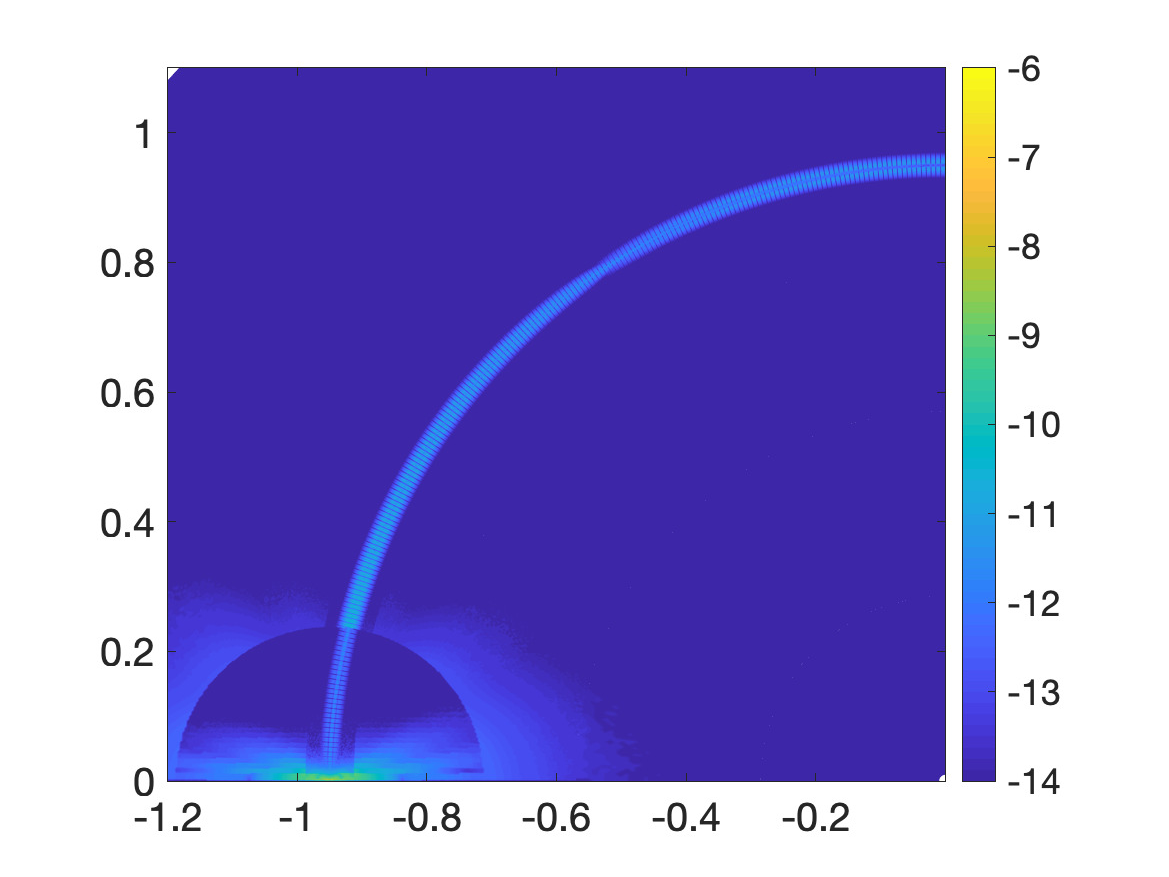
\includegraphics[trim=40 20 40 10, clip, width=2.5truein]{figs/fig400c4}\\
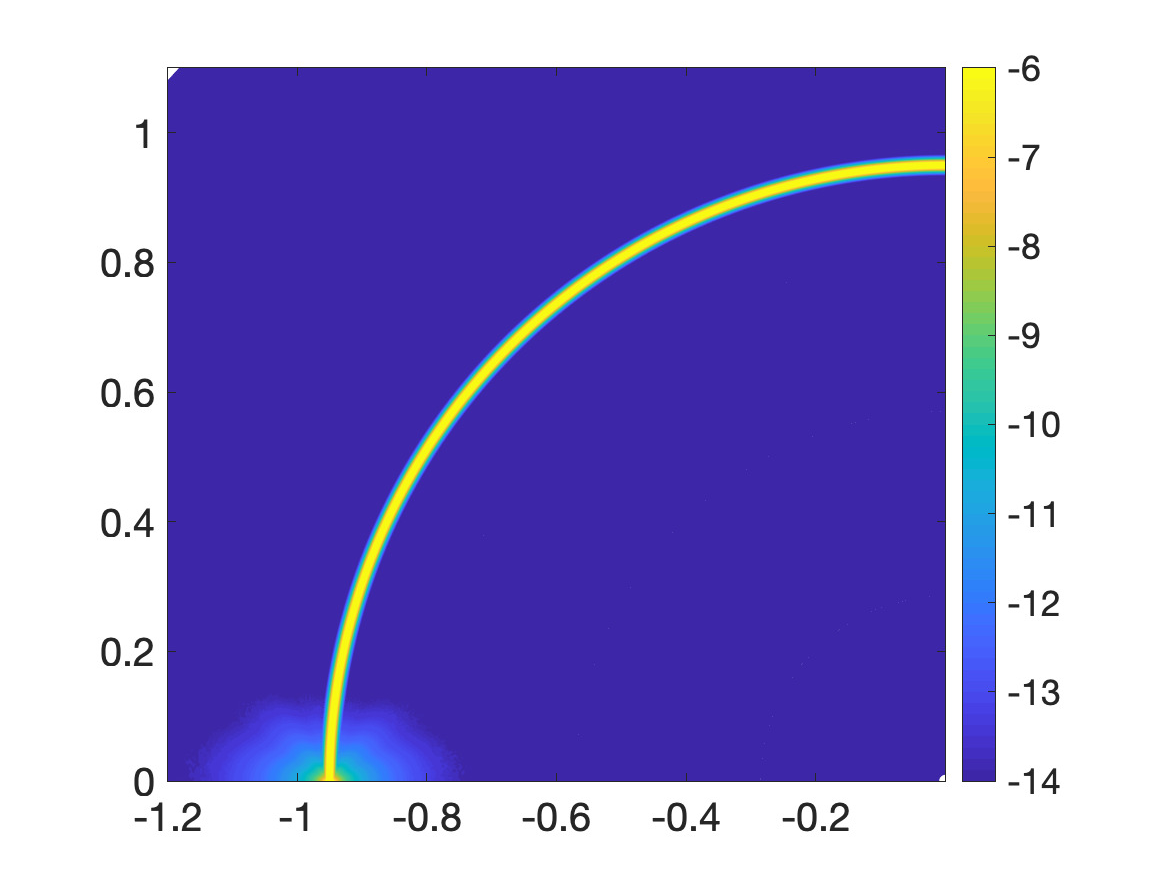
\includegraphics[trim=40 20 40 10, clip, width=2.5truein]{figs/fig800a4} 
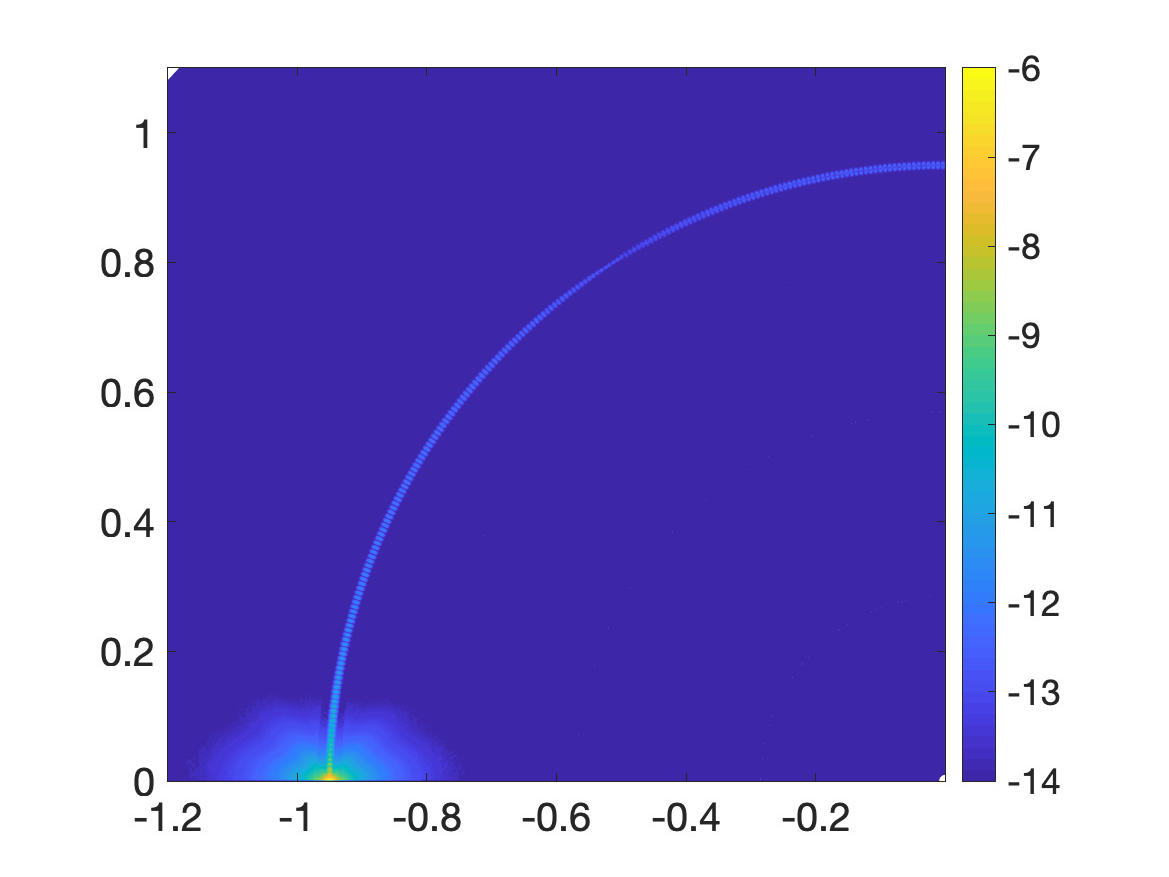
\includegraphics[trim=40 20 40 10, clip, width=2.5truein]{figs/fig800b4} 
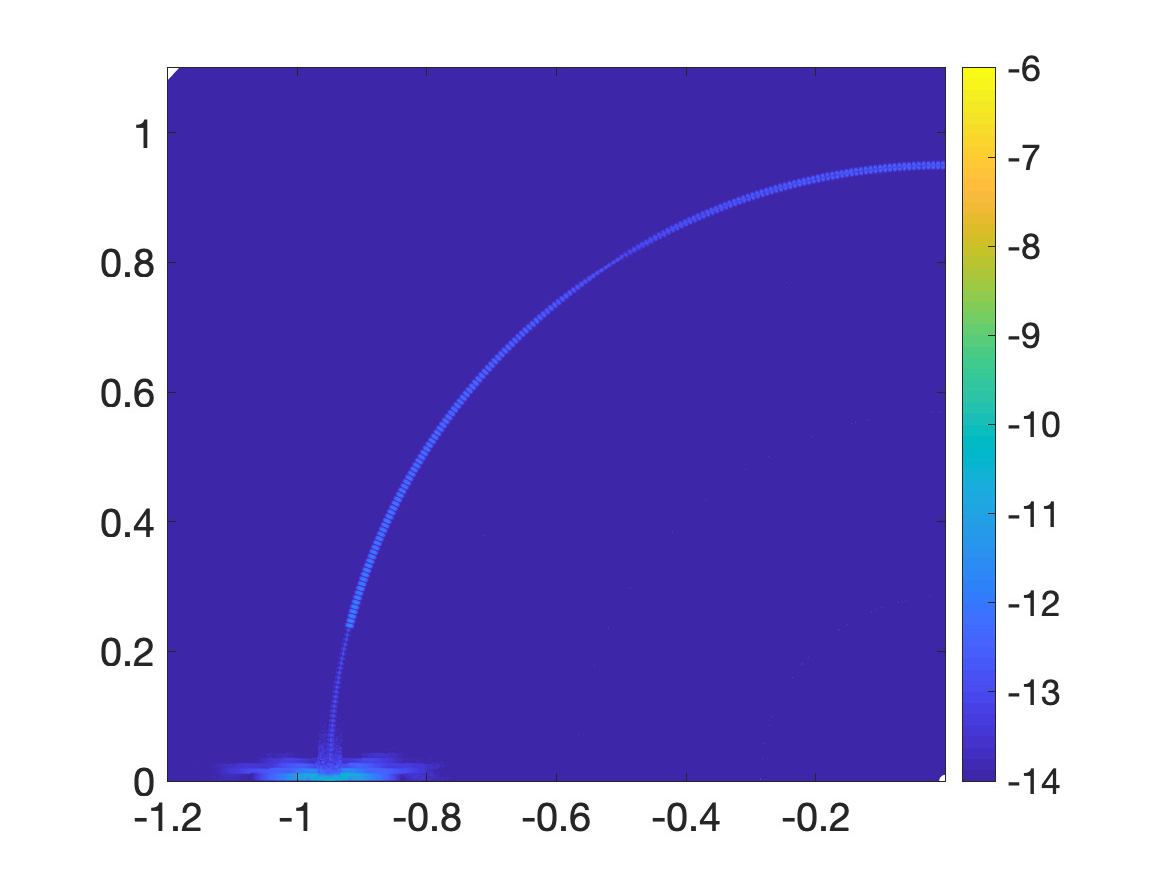
\includegraphics[trim=40 20 40 10, clip, width=2.5truein]{figs/fig800c4} 
\vfill
\noindent
The rows, top to bottom, show results using $n=100,200,400,800$.\\
The columns, left to right, show errors obtained with $T[G]$, $T[G]+E[H]$, $T[G]+E[H]+E[B]$.
\end{document}


